\section{Simulaciones}
\subsection{Simulación con valores teóricos}
Se simuló el circuito con todos los componentes calculados:
\begin{figure}[!h]
    \centering
    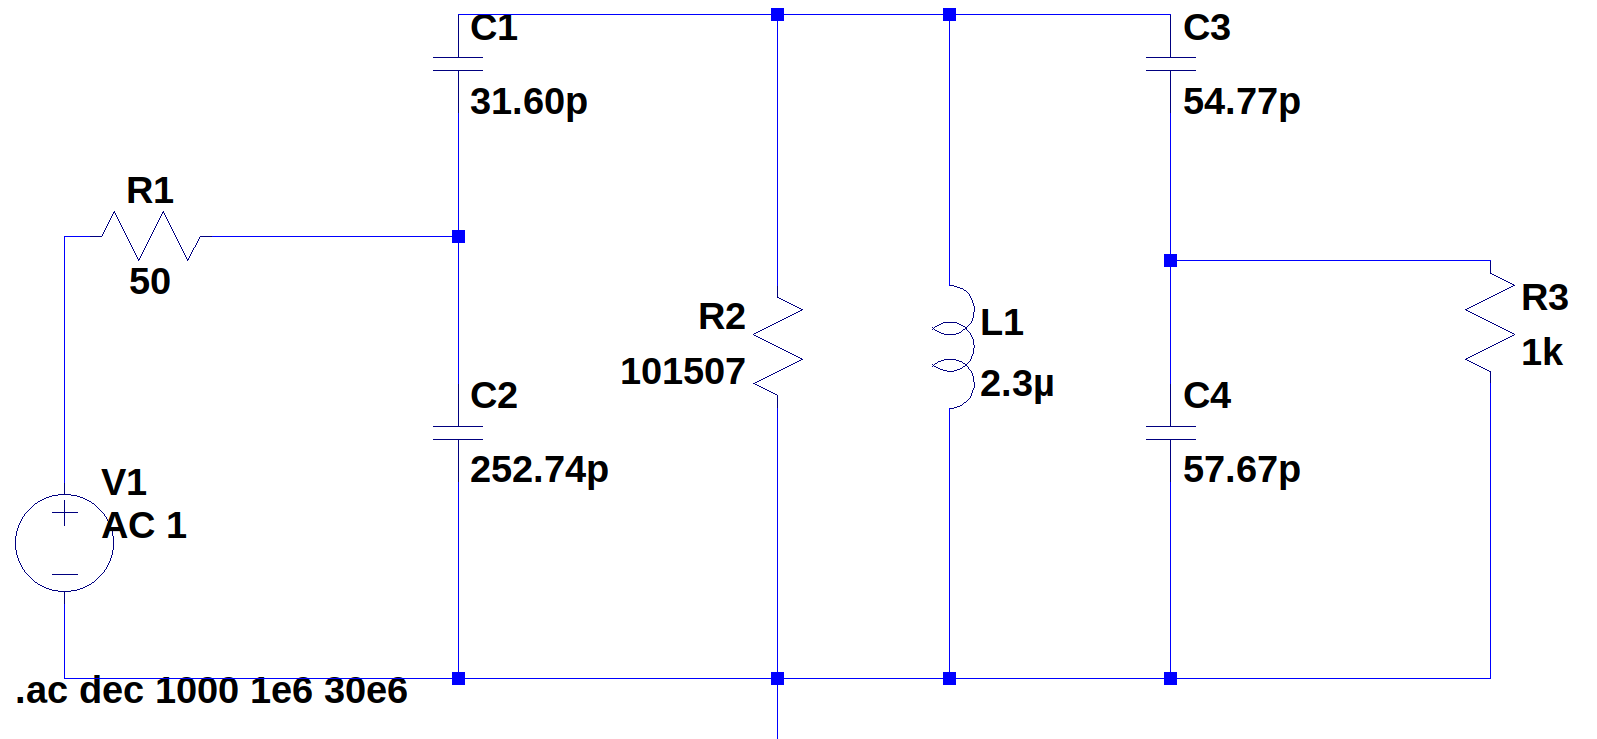
\includegraphics[scale=0.2]{Imagenes/Circuito teorico.png}
    \caption{Esquemático del circuito teórico en LTspice}
    \label{fig:Circteo}
\end{figure}

\begin{figure}[!h]
    \centering
    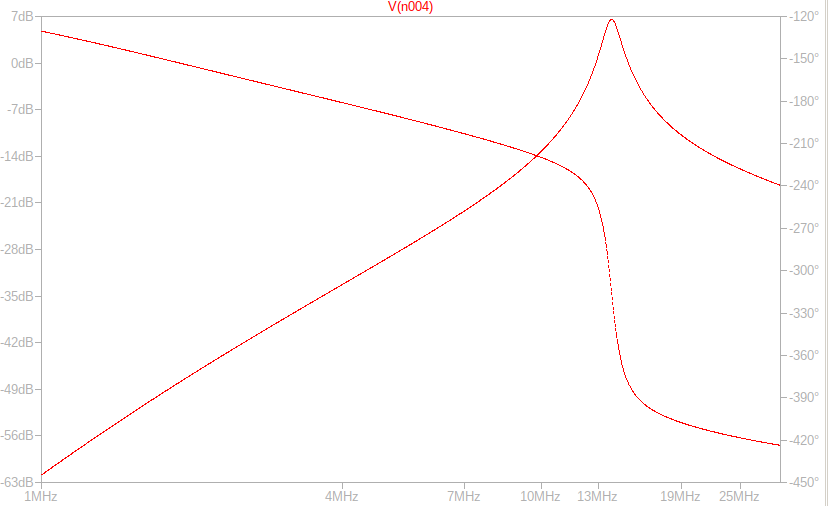
\includegraphics[scale=0.4]{Imagenes/db_f.png}
    \caption{Diagrama de Bode de amplitud y fase}
    \label{fig:Circteo}
\end{figure}

\newpage
\begin{figure}[!h]
    \centering
    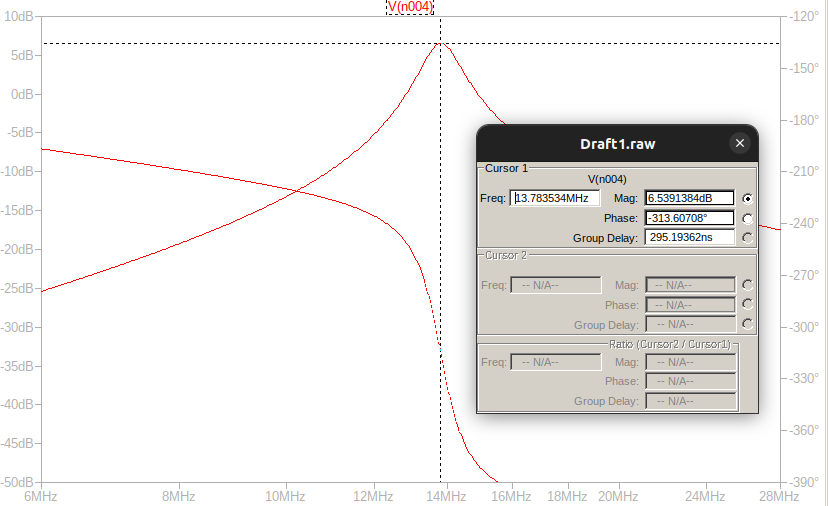
\includegraphics[scale=0.4]{Imagenes/dbzoom.png}
    \caption{Diagrama de Bode ampliado en \(f_o\)}
    \label{fig:Circteo2}
\end{figure}
Se observa que la frecuencia \(f_0\) es aproximadamente 13,78 MHz y se tiene una amplitud de 6,53 dB. Lo siguiente es medir su \(BW\) donde la amplitud caiga 3 dB :
\begin{figure}[!h]
    \centering
    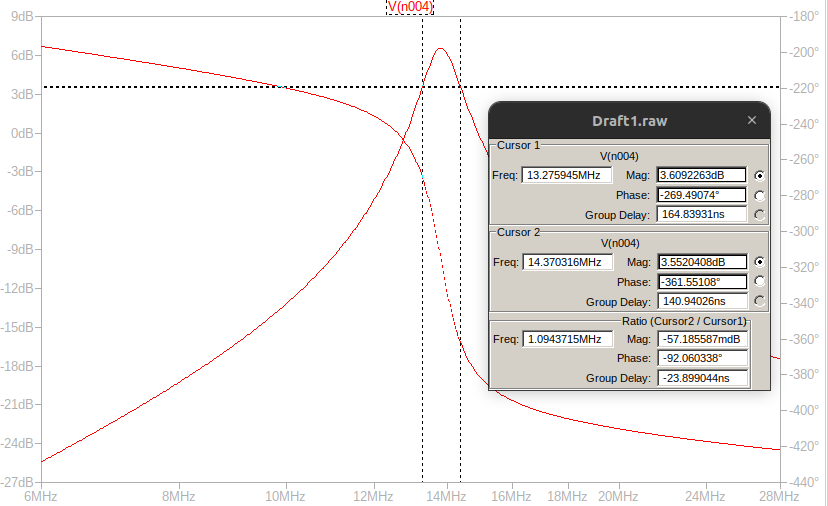
\includegraphics[scale=0.4]{Imagenes/BW.png}
    \caption{Medición del \(BW\)}
    \label{fig:bw}
\end{figure}

Si se observa la figura 12, de esta se puede extraer que el \(BW = 1,1\) MHz aproximadamente. 
\newpage
\subsection{Simulación con valores de capacitores comerciales conseguidos.}
Para los valores comerciales que se pudieron conseguir, se simuló el circuito con dichos valores de capacitores para observar como variaba la \(f_o\):
\begin{figure}[!h]
    \centering
    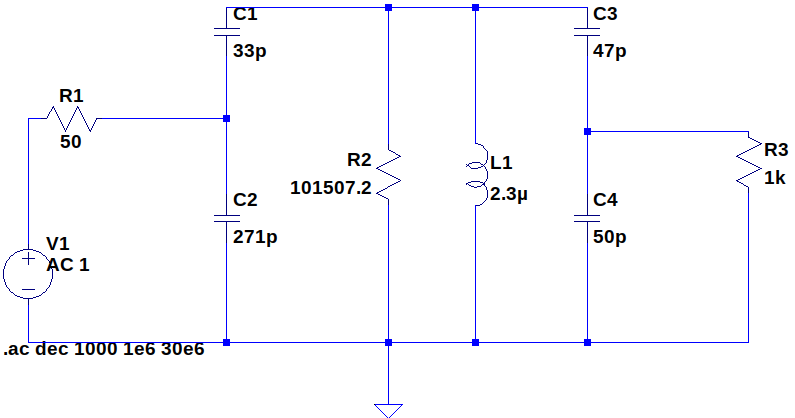
\includegraphics[scale=0.4]{Imagenes/Circreal.png}
    \caption{Esquemático de circuito con capacitores comerciales}
    \label{fig:bw}
\end{figure}

\begin{figure}[!h]
    \centering
    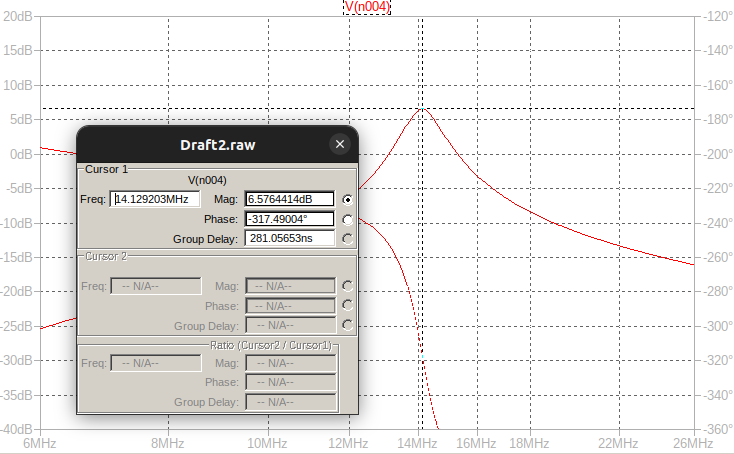
\includegraphics[scale=0.4]{Imagenes/Circreal_bode.png}
    \caption{Diagrama de Bode }
    \label{fig:bw}
\end{figure}
La frecuencia de resonancia central \(f_o\) es 14,13 MHz, la amplitud y el \(BW\) son prácticamente los mismos. Por ultimo, se calcula el \(Q_c\) mediante la ecuación (3): 
\begin{equation}
    Q_c = \frac{14,13 \text{MHz}}{1,1 \text{MHz}} = 12,84 
\end{equation}


